%************************************************
\chapter{Design}\label{ch:design}
%************************************************
\glsresetall % Resets all acronyms to not used

\lipsum[9]


%************************************************
\chapter{Implementation}\label{ch:implementation} % $\mathbb{ZNR}$
%************************************************
\glsresetall % Resets all acronyms to not used

\section{Radio Data System}

Demodulation of the \ac{RDS} signal is first done in Octave in order to
evaluate the demodulation algorithm. The octave implementation
also helps by providing reference data of the different stages
of demodulation. 

\subsection{RDS modulation scheme}

\ac{RDS} uses \ac{BPSK} with Manchester encoding. The signal is
transmitted with an offset of 57 kHz relative to the center frequency
of the mono audio signal (baseband). The 19 kHz pilot tone of wideband \ac{FM}
can therefore be used to retrieve the \ac{RDS} carrier by multiplying
it with itself 3 times. The complete FM spectrum can be seen in
\autoref{fig:quad_demod_spectrum}.

After the \ac{RDS} baseband signal has been retrieved from the \ac{FM} signal
there are multiple ways of demodulating the \ac{BPSK} modulation. A sophisticated
approach tries to recover the phase synchronised \ac{RDS} carrier from the
signal by using e.g. a form of \ac{PLL} or Costas Loop. The symbols can then
be extracted by multiplying the carrier with the modulated signal and apply
a threshold operation to get bits.

\subsection{Evaluation in Octave}


\begin{figure}
\subfloat[Spectrum of the captured signal]{%
  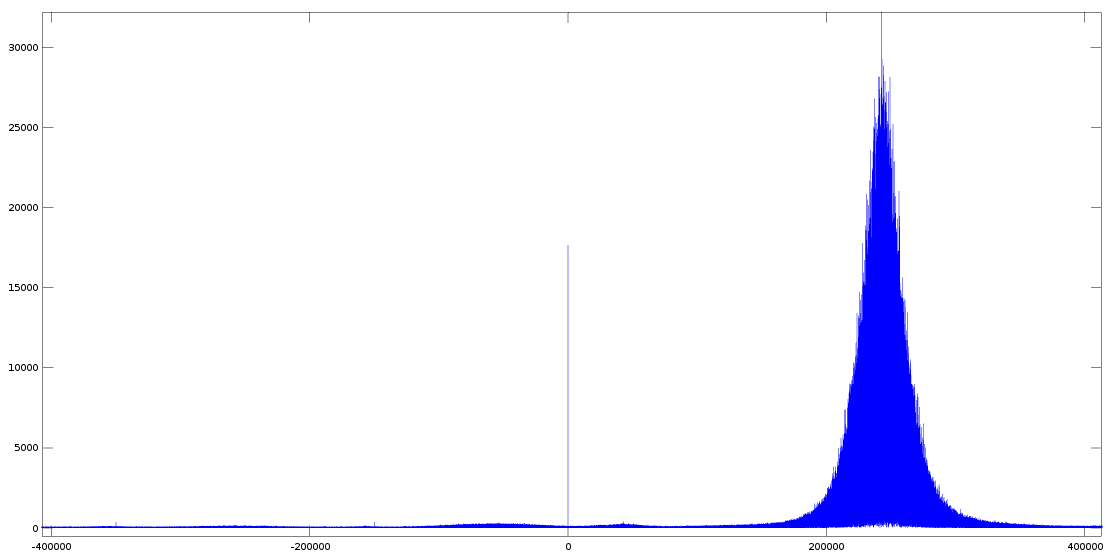
\includegraphics[clip,width=1\linewidth]{gfx/rds/raw_signal_spectrum.png}%
}

\subfloat[Spectrum after downmixing and filtering]{%
  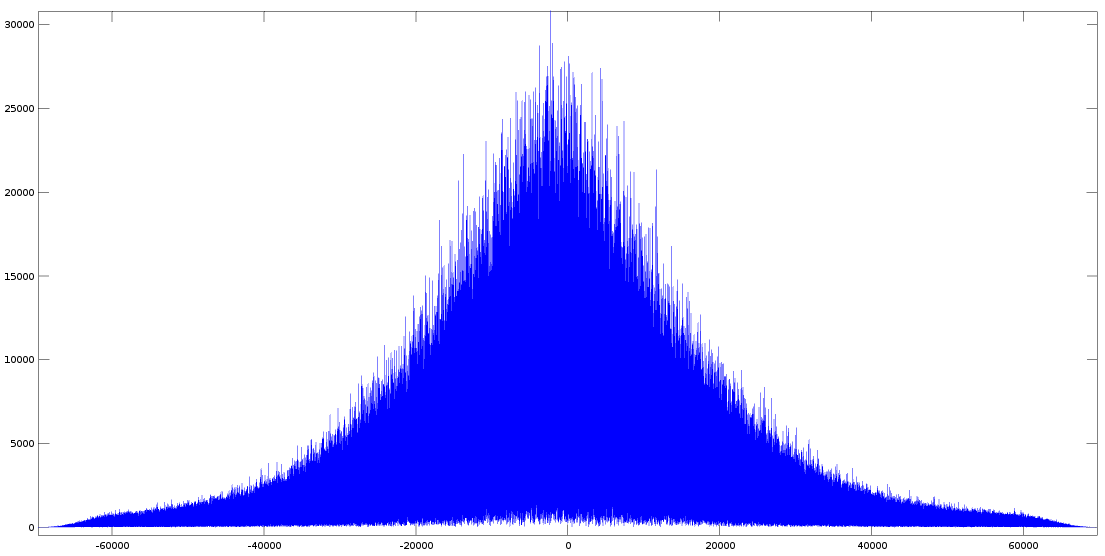
\includegraphics[clip,width=1\linewidth]{gfx/rds/fm_baseband_filtered_spectrum.png}%
}
\caption{FM Modulated Signal}

\end{figure}


\begin{figure}
\subfloat[Signal spectrum after FM demodulation]{%
  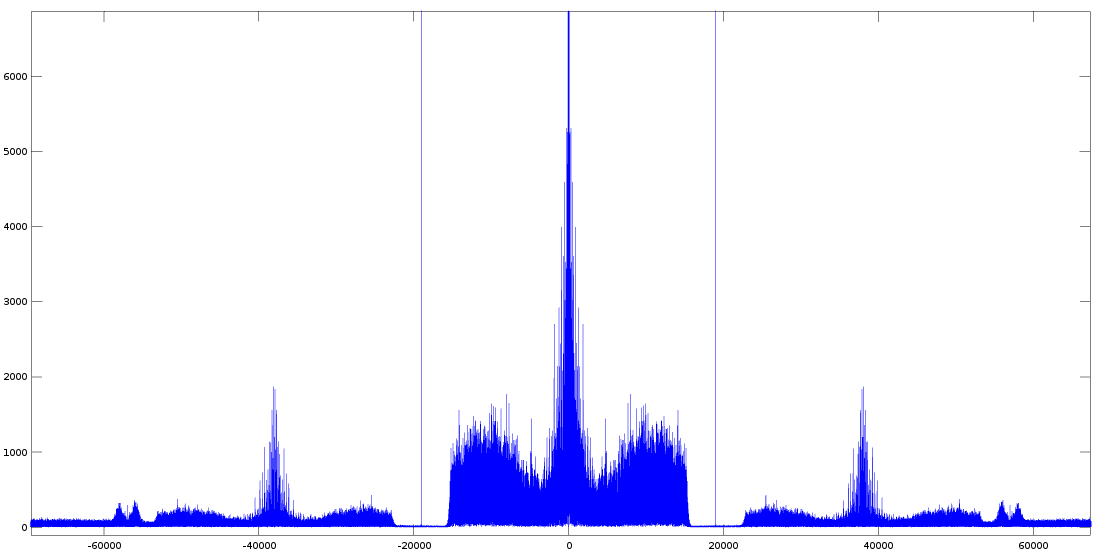
\includegraphics[clip,width=1\linewidth]{gfx/rds/quad_demod_spectrum.png}%
  \label{fig:quad_demod_spectrum}
}

\subfloat[RDS baseband spectrum after downmixing]{%
  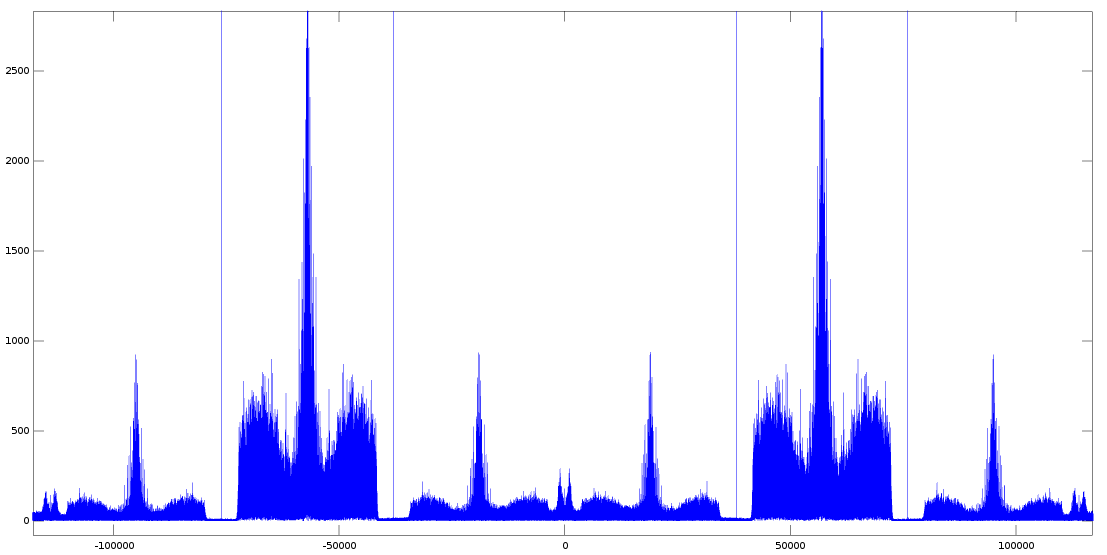
\includegraphics[clip,width=1\linewidth]{gfx/rds/rds_baseband_unfiltered_spectrum.png}%
}

\subfloat[RDS baseband spectrum after filtering]{%
  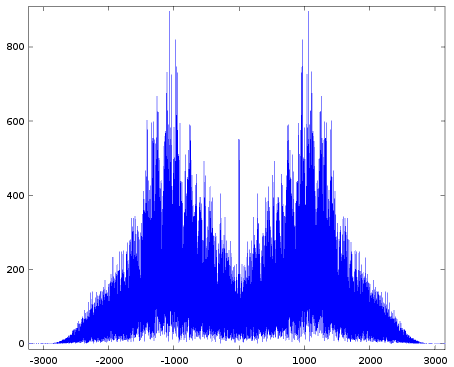
\includegraphics[clip,width=1\linewidth]{gfx/rds/rds_baseband_spectrum.png}%
}
\caption{Extracting the RDS signal from the FM signal}

\end{figure}

\begin{figure}
	\centering
	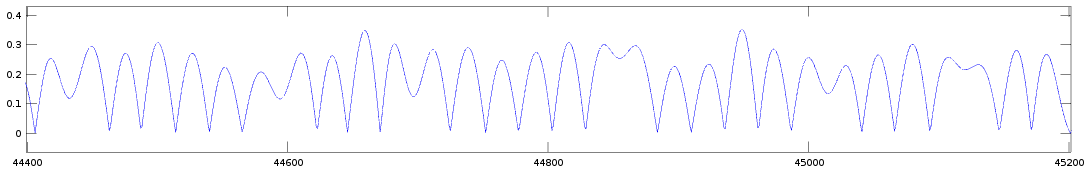
\includegraphics[width=1\linewidth]{gfx/rds/rds_magnitude_waveform.png}
	\caption{RDS waveform after take the absolute values}
	\label{fig:rds_waveform}
\end{figure}


\subsection{Android Implementation}



\subsection{Problems}


%************************************************
\chapter{Evaluation}\label{ch:evaluation} % $\mathbb{ZNR}$
%************************************************
\glsresetall % Resets all acronyms to not used

\lipsum[5]
